\section{Introduzione}

    \begin{definition}[Base di Dati]
        Una base di dati è un insieme organizzato di dati utilizzati per il supporto allo svolgimento di attività.
    \end{definition}

    \paragraph*{Struttura dei Dati}
    I dati sono organizzati in insiemi strutturati che possono presentare fra loro delle relazioni. Tuple che rappresentano dati nello stesso insieme devono essere omogenee ed univoche.

    \begin{definition}[Sistema Informativo]
        Un sistema informativo è una combinazione di risorse umane e/o materiali e procedure organizzate per
        la \textcolor{purple}{raccolta}, l'\textcolor{purple}{archiviazione}, l'\textcolor{purple}{elaborazione}
        e lo \textcolor{purple}{scambio} di informazioni necessarie ad un'attività, le quali possono essere classificate in:
        \begin{itemize}
            \item Informazioni di servizio (operative).
            \item Informazioni di controllo (pianificazione e gestione).
            \item Informazioni di governo (pianificazione strategica).
        \end{itemize}
        \begin{figure}[h]
            \centering
            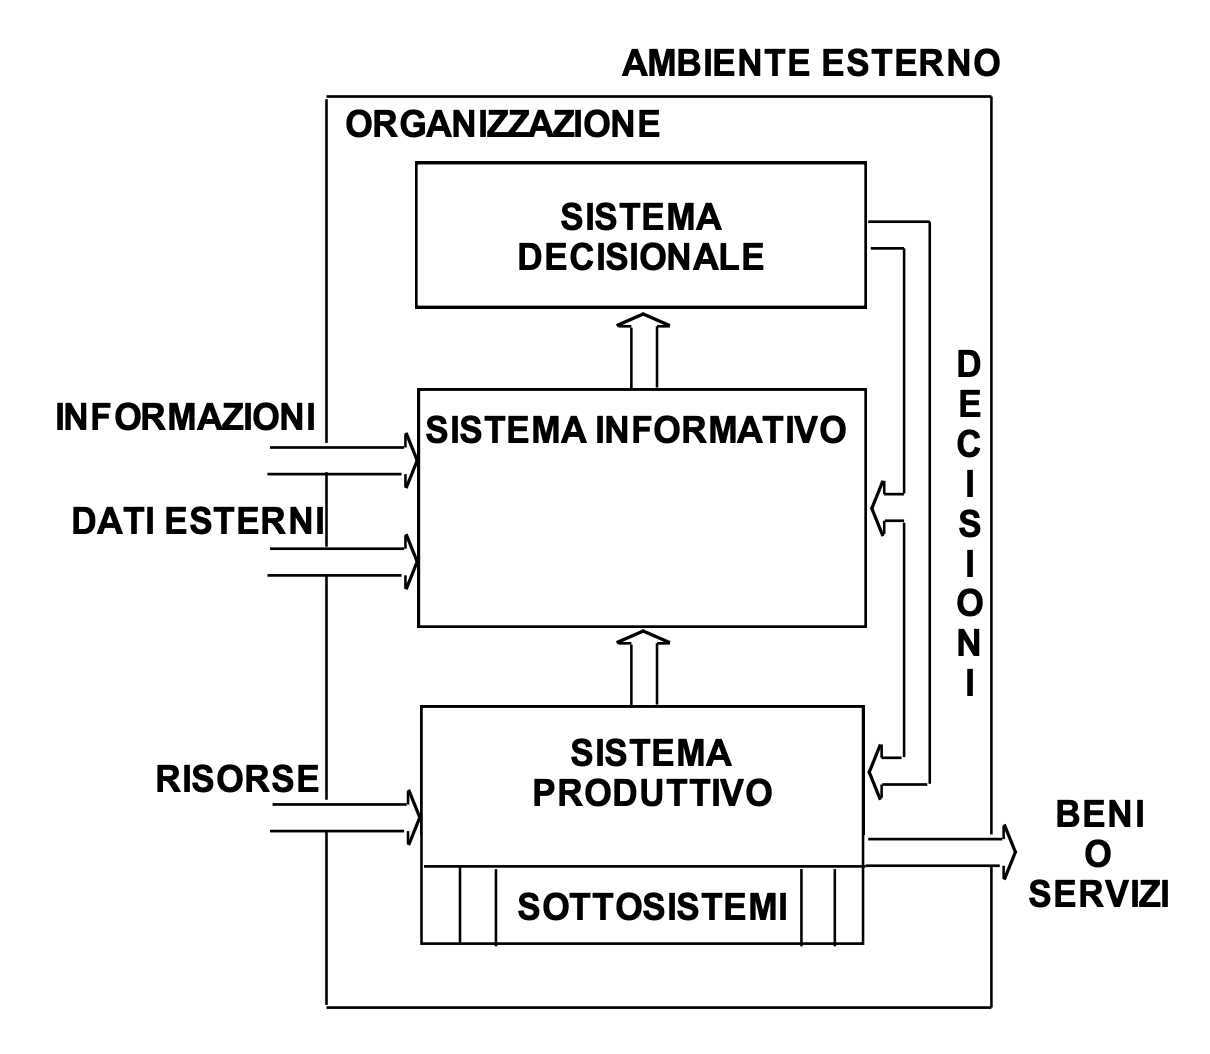
\includegraphics[scale=0.5]{img/sistema_informativo.png}
            \caption{Esempio di sistema informativo}
        \end{figure}
    \end{definition}

    \begin{definition}[Sistema Informativo Automatizzato]
        Un sistema informativo automatizzato è una parte del sistema informativo che permette di implementare le procedure
        che si occupano della gestione delle informazioni usando un sistema informatico.
    \end{definition}

    \begin{definition}[Sistema Informatico]
        Un sistema informatico è l'insieme delle tecnologie a supporto per le attività di un'organizzazione.
        Si possono classificare in:
        \begin{itemize}
            \item \textbf{\textcolor{purple}{Sistemi informatici operativi}}: questi sistemi si utilizzano per svolgere le normali attività dell'azienda
                per la fruizione del suo bene o servizio, e per la gestione interna dei singoli reparti dell'azienda.
                Le operazioni sui dati in questo sistema sono di tipo \textcolor{purple}{OLTP} (\emph{On-Line Transaction Processing})
                e prevedono elaborazioni semplici che coinvolgono pochi dati che vengono aggiornati molto frequentemente.
            \item \textbf{\textcolor{purple}{Sistemi informatici direzionali}}: i dati sono organizzati in \emph{Data Warehouse}
                che consentono di aiutare l'azienda nei processi di controllo delle prestazioni e di decisione manageriale.
                Le elaborazioni su questo tipo di sistema si chiamano \textcolor{purple}{OLAP} (\emph{On-Line Analytical Processing})
                e prevedono l'utilizzo di una grande mole di dati che sono per lo più storici. In questo caso i dati vengono aggiornati
                molto raramente, ma su di essi vengono svolte molte operazioni, anche da un punto di vista multidimensionale, ovvero
                vengono incrociati più dati per analizzare le informazioni ottenute sotto molteplici punti di vista.
        \end{itemize}
    \end{definition}

    \begin{definition}[DBMS]
        Un \emph{Database Management System} è un sistema che garantisce
        il controllo e la gestione di dati per renderli accessibili agli utenti opportuni in base ai loro privilegi.
        Il DBMS fornisce anche dei linguaggi che permettono di definire lo \textcolor{purple}{schema} di un database, di scegliere le \textcolor{purple}{strutture dati}
        opportune per la memorizzazione dei dati, di rispettare i \textcolor{purple}{vincoli} per ogni tipo di dato e di poter \textcolor{purple}{modificare} e
        \textcolor{purple}{interrogare} il database.
    \end{definition}

    \paragraph*{Metadati} All'interno del database sono anche memorizzati dei metadati che si riferiscono agli utenti
    e allo schema utilizzato dal database stesso. Anche i metadati possono essere interrogati e modificati.